\documentclass[tikz,border=2pt]{standalone}
\usepackage{amsmath,amssymb}
\usepackage{tikz}

\begin{document}
% An even number of yes decisions among y1, y2, y3: the sum must be 0 or 2, enforced by
% y1 + y2 + y3 = 2x with a binary x.
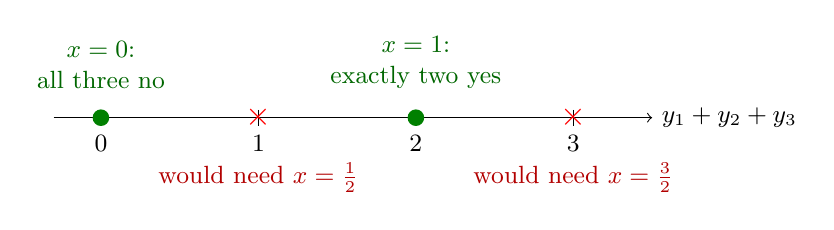
\begin{tikzpicture}[every node/.style={font=\small}]
	\draw[->] (-0.6,0) -- (7.0,0) node[right] {$y_1+y_2+y_3$};
	\foreach \x in {0,1,2,3} {\draw ({2*\x},0.1) -- ({2*\x},-0.1) node[below] {$\x$};}
	\fill[green!50!black] (0,0) circle (3pt); \fill[green!50!black] (4,0) circle (3pt);
	\node[red, font=\large] at (2,0) {$\times$}; \node[red, font=\large] at (6,0) {$\times$};
	\node[green!40!black, anchor=south, align=center] at (0,0.25) {$x=0$:\\ all three no};
	\node[green!40!black, anchor=south, align=center] at (4,0.25) {$x=1$:\\ exactly two yes};
	\node[red!70!black, anchor=north] at (2,-0.45) {would need $x=\tfrac12$};
	\node[red!70!black, anchor=north] at (6,-0.45) {would need $x=\tfrac32$};
	\end{tikzpicture}
\end{document}
